\documentclass[10pt]{beamer}

\usetheme{Montpellier}
\usecolortheme{whale}

\usepackage[T1]{fontenc}
\usepackage{lmodern}

\usepackage{mathtools}
\usepackage[binary-units]{siunitx}
\usepackage{amsmath}
\usepackage{listings}
\usepackage{mdframed}
\usepackage{adjustbox}
\usepackage{minted}
\usepackage{xcolor}

\usepackage{parskip}
\usepackage{substr}
\usepackage{hyperref}
\usepackage{etoolbox}
\usepackage{tipa}
\usepackage{cprotect}
\usepackage{booktabs}
\usepackage{silence}
\usepackage[backend=biber, style=ieee]{biblatex}
\usepackage[english,ngerman]{babel}
\usepackage{csquotes}

\definecolor{lg}{gray}{0.95}
\hypersetup{colorlinks = true, urlcolor=blue, linkcolor=white}
\WarningFilter{biblatex}{Patching footnotes failed}

\renewcommand*{\bibfont}{\tiny}
\renewcommand{\subsectionname}{AA}

\bibliography{resources.bib}

\title{\textbf{Operating Systems}}
\subtitle{Tutorial 5}
\author{Fabian Klopfer}
\date{\today}

\defbeamertemplate{subsection page}{mine}[1][]{%
  \begin{centering}
    {\usebeamerfont{subsection name}\usebeamercolor[fg]{subsection name}#1}
    \vskip1em\par
    \begin{beamercolorbox}[sep=12pt,center]{part title}
      \usebeamerfont{subsection title}\insertsubsection\par
    \end{beamercolorbox}
  \end{centering}
}

\defbeamertemplate{section page}{mine}[1][]{%
  \begin{centering}
    {\usebeamerfont{section name}\usebeamercolor[fg]{section name}#1}
    \vskip1em\par
    \begin{beamercolorbox}[sep=12pt,center]{part title}
      \usebeamerfont{section title}\insertsection\par
    \end{beamercolorbox}
  \end{centering}
}

\setbeamertemplate{section page}[mine]
\setbeamertemplate{subsection page}[mine]

\begin{document}
\frame{\titlepage}


\begin{frame}{Intro}
\begin{itemize}
 \item Pingo Polls
\end{itemize}
\end{frame}

\section*{Exercise Sheet 4}
\frame{\sectionpage}
\subsection*{Exercise 1}
\frame{\subsectionpage}
\begin{frame}[allowframebreaks, fragile]{Exercise 1}
    \begin{enumerate}
		\item Name six mechanisms for memory management.\\
            \alert{For example: Address spaces, swapping, virtual memory, paging, segmentation, compression.}
            
		\item What is swapping and which problem does it solve?\\
            \alert{
            \begin{itemize}
            \item Using disk space to store process memory to RAM of currently not used processes. 
            \item Solves the problem of having not enough RAM for all processes.
            \end{itemize}
            }
            
		\item Which problem does virtual memory solve? \\
            \alert{The problem of requiring more RAM than available.}
            
		\item What is the task of the Memory Management Unit (MMU) with respect to memory management? \\
            \alert{Translates virtual to physical addresses.}
		
		\item For which computing systems (e.g. mainframes, personal computers, $\ldots$) is virtual memory not needed, and why? \\
            \alert{Where hardware and software is known and fixed. \\
            Small scale systems e.g. sensor nodes, special processors (e.g. DSPs). \\
            Pros: Simpler MM, smaller OS.}
		
		\item Give another example for accessing memory that causes a ``segmentation fault''. \\
            \alert{Accessing another processes memory, writes to read-only regions.}
			
		\item Does swapping write all the memory reserved by the operating system for a process to disk? \\
            \alert{Only the actually used regions.}
		
	\end{enumerate}
\end{frame}

\subsection*{Exercise 2}
\frame{\subsectionpage}
\begin{frame}[allowframebreaks, fragile]{Exercise 2}
    \begin{enumerate}
		\item Why does the $O(1)$ scheduling algorithm have constant runtime? \\
			\alert{
			\begin{enumerate}
				\item Get next process to run: \\
					Identify non-empty highest priority queue, i.e. find first set bit in \textit{active} array. $\Rightarrow \mathcal{O}(1)$.
				\item%
                    Remove from run queue: \\
					Process doesn't have to be looked up (it's the active one, right?), i.e. only insert it into a queue. $\Rightarrow \mathcal{O}(1)$.
				\item%
					Switch \textit{active} with \textit{expired}:
					Swap the pointers. $\Rightarrow \mathcal{O}(1)$.
			\end{enumerate}
			}
		\item For computing systems with multiple CPUs, Linux maintains a run queue for each CPU.
			State an efficiency advantage of this solution compared to a single run queue for all CPUs.
			\alert{\begin{itemize}
			        \item Caching
			        \item Less synchronization effort
			       \end{itemize}
}
		\item Why does CFS use a red-black tree instead of a list?
		\alert{No linked list look up ($\mathcal{O}(n)$) but tree look ups ($\mathcal{O}(\log(n)$)}
	\end{enumerate}
\end{frame}

\subsection*{Exercise 3}
\frame{\subsectionpage}
\begin{frame}[allowframebreaks, fragile]{Exercise 3}
    Write a function \mintinline{c}{void string_reverse_inplace(char *s)} which reverses strings in-place. $[\dots]$ \\ \vspace{0.6cm}
    \adjustbox{varwidth=\textwidth}{
        \inputminted[autogobble, fontsize=\scriptsize]{c}{code/str_rev.c}
    }
\end{frame}

\subsection*{Exercise 4}
\frame{\subsectionpage}
\begin{frame}[allowframebreaks, fragile]{Exercise 4}
    \begin{enumerate}
        \item Write a function that swaps two \mintinline{c}{int} variables in-place without using any local variables.   \\ \vspace{0.6cm} \adjustbox{varwidth=\textwidth}{
        \inputminted[autogobble, fontsize=\scriptsize]{c}{code/bit_swap.c}
    }
    \vspace{0.6cm}
    
        \item Prove the correctness of your approach.
    \end{enumerate}

    \framebreak
    \alert{
    \begin{enumerate}
     \item Version:
     Let $a,\ b$ variables with binary base. Let $t = a \text{ XOR } b$. Thus $t$ is $0$ at place $i$ if $a_i = b_i$ and 1 otherwise. \\
 \[ t \text{ XOR } a = b \]
 \[ t \text{ XOR } b = a \]
 is to be proven. Starting with the first conjecture.
 \[ t \text{ XOR } a = a \text{ XOR } b \text{ XOR } a \]
 Using that XOR is associative, commutative and self-inverse, we get:
 \[ a \text{ XOR } a \text{ XOR } b  = 0 \text{ XOR } b = b \]
 Similarly for the second one.
 \framebreak
 
 \item Version: As Only bits-wise ops used, sufficient to show correctness for one bit (more bits follow inductively):\\
 
\begin{center}
 			\medskip
			\begin{tabular}{@{}ccccc@{}}
				\toprule
				\mintinline{c}{ab} & \mintinline{c}{a^=b} & \mintinline{c}{b^=a} & \mintinline{c}{a^=b} \\
				\midrule
				00 & 00 & 00 & 00 \\
				01 & 11 & 10 & 10 \\
				10 & 10 & 11 & 01 \\
				11 & 01 & 01 & 11 \\
				\bottomrule
			\end{tabular}
        \end{center}
    \end{enumerate}
    }

		
\end{frame}

\subsection*{Exercise 5}
\frame{\subsectionpage}
\begin{frame}[allowframebreaks, fragile]{Exercise 5}
	\begin{enumerate}
		\item%
			How long does it take to compress \SI{4}{\gibi\byte} of memory when both reading and writing a 32-bit word each take \SI{4}{\nano\s}?
			Assume that the entire memory must be compressed, e.g., because the beginning of memory is in a gap and the end of memory is allocated to a process.
			\alert{
			 \[ 2 \cdot \frac{4 \text{ ns}}{32 \text{ bit}} = 2 \frac{\text{ns}}{\text{bytes}} \]
            \[ 4 \text{ GiB} \cdot 2 \frac{\text{ns}}{\text{bytes}} = 2^{32} \text{ bytes} \cdot 2 \cdot 10^{-9}  \frac{\text{s}}{\text{bytes}} \]
            \[ 2^{33} \cdot 10^{-9} \text{ s} = 8.589934592 \text{ s} \]
            }
		\item%
			Swapping caused the following gaps in main memory, given in ascending address order:
			\SI{10}{\mega\byte}, \SI{4}{\mega\byte}, \SI{20}{\mega\byte}, \SI{18}{\mega\byte}, \SI{7}{\mega\byte}, \SI{11}{\mega\byte}, \SI{12}{\mega\byte}, \SI{15}{\mega\byte}.
			Which gaps do the First Fit, Next Fit, Best Fit and Worst Fit algorithms select
			if memory segments of size
			\SI{12}{\mega\byte}, \SI{10}{\mega\byte}, \SI{9}{\mega\byte} 
			are successively requested for processes? \\
			\begin{center}
			\alert{
			\begin{tabular}[t]{@{}lccc@{}}
				\toprule
				Algorithmus & \SI{12}{\mega\byte} & \SI{10}{\mega\byte} & \SI{9}{\mega\byte} \\
				\midrule
				First Fit & 20 & 10 & 18 \\
				Next Fit  & 20 & 18 & 11 \\
				Best Fit  & 12 & 10 & 11 \\
				Worst Fit & 20 & 18 & 15 \\
				\bottomrule
			\end{tabular}
			}
						\end{center}
	\end{enumerate}
\end{frame}

\subsection*{Exercise 6}
\frame{\subsectionpage}
\begin{frame}[allowframebreaks, fragile]{Exercise 6}
    Write a program that reads text from standard input and outputs a histogram of word lengths. \\
	 \alert{
        Too long for slides, show in editor.
	 }
\end{frame}

    
\section*{Exercise sheet 5}
\frame{\sectionpage}
\begin{frame}[allowframebreaks, fragile]{}
 \begin{figure}
           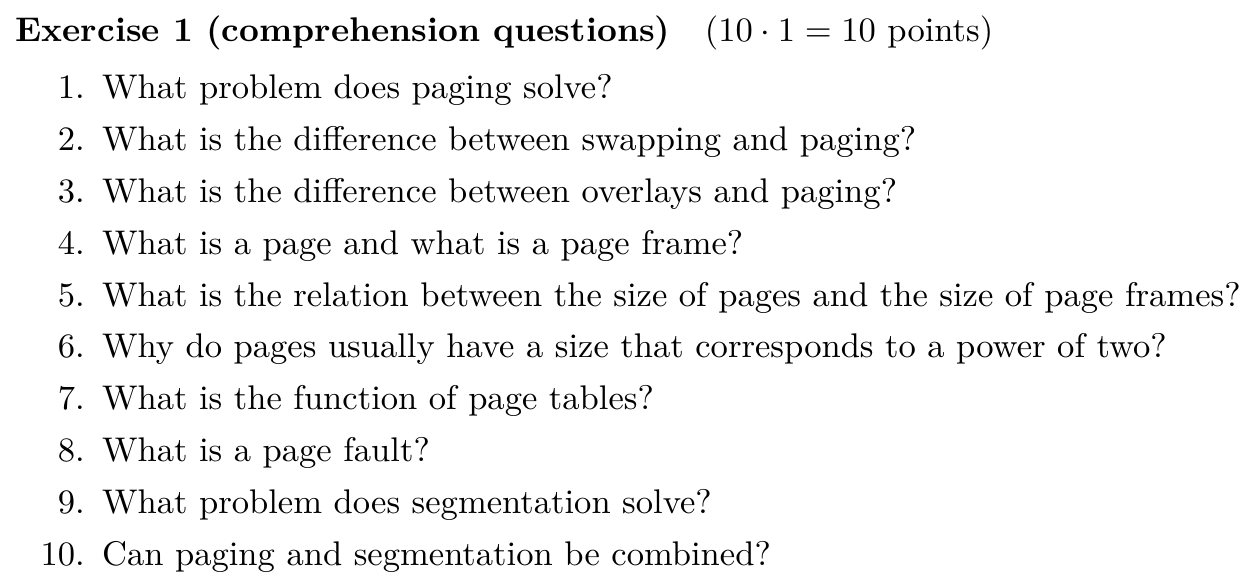
\includegraphics[keepaspectratio, width=\textwidth, height=\textheight-2\baselineskip-2\baselineskip]{img/100_ex5.png} \\
        \end{figure}
        \begin{itemize}
         \item All in the book, mostly in the paging chapter
        \end{itemize}
        \framebreak
        
  \begin{figure}
          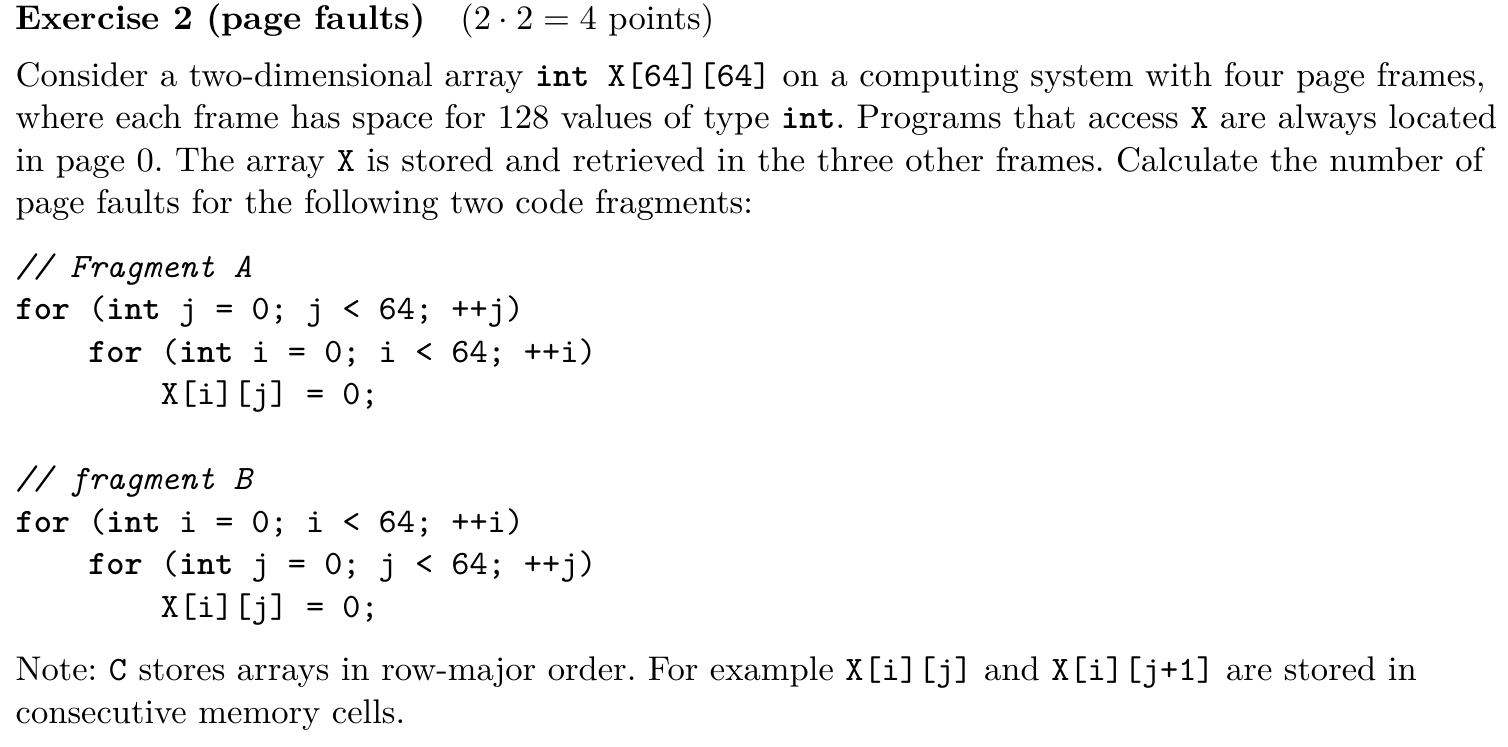
\includegraphics[keepaspectratio, width=\textwidth, height=\textheight-2\baselineskip-2\baselineskip]{img/101_ex5.png} \\
        \end{figure}
        \begin{itemize}
         \item How many iterations can be done with the contents of one page?
         \item Mind the iteration order: The \textit{inner} loop decides how many items can be read from one page.
        \end{itemize}
        \framebreak
        
         \begin{figure}
          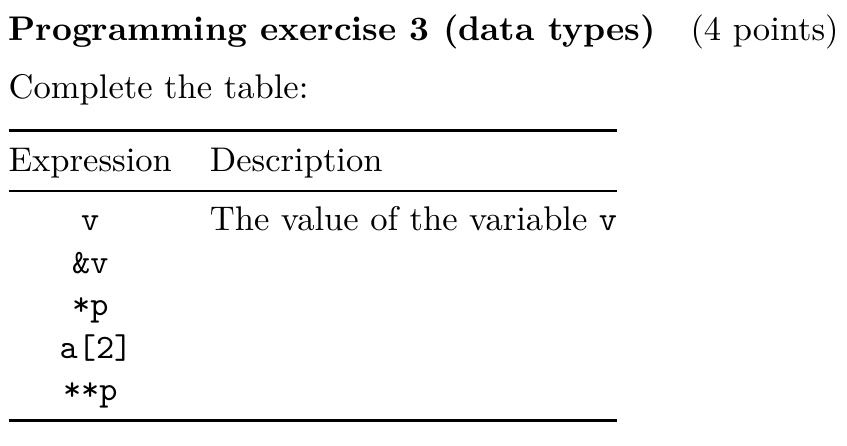
\includegraphics[keepaspectratio, width=0.8\textwidth, height=0.8\textheight-2\baselineskip-2\baselineskip]{img/102_ex5.png} \\
        \end{figure}
        \begin{itemize}
         \item Check out the C Programming Language \autocite{kernighan2006c}, chapter 5 (especially 5.3 (3 pages)).
         \item Remember \mintinline{c}{&} gives you the address of a value, \mintinline{c}{*} gives you the value at an address
        \end{itemize}
        \framebreak 
        
         \begin{figure}
          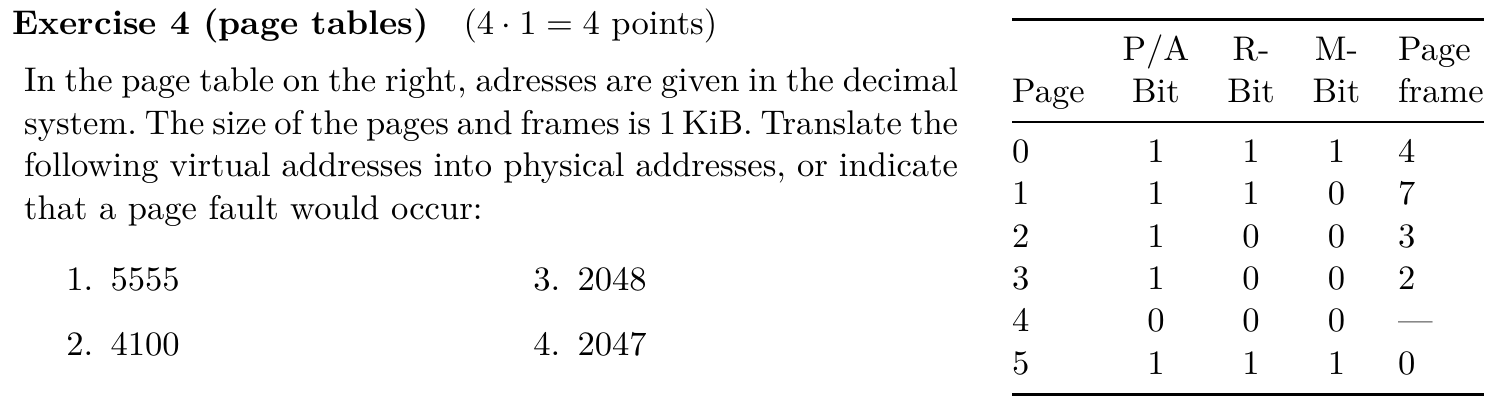
\includegraphics[keepaspectratio, width=\textwidth, height=\textheight]{img/103_ex5.png} \\
        \end{figure}
        \begin{itemize}
        \item 6 Pages, next power of 2 is $2^3 = 8 \Rightarrow 3$ Bits for pages
        \item 1KiB are $2^?$
        \item $3 + ? =$ bits of a virtual address 
        \item Use bit masks, logical and \& shifts to extract page ID and offset
        \item Use bit shift and logical or to construct physical address from frame and offset
        \framebreak
         \item Example: $1025_{10} = 0010000000001_2$. \\ \vspace{0.4cm}
        Page ID = (Bit Mask \& Virtual Address) $>>$ Offset length
            \[ (1110000000000_2 \& 00100000010001_2) >> 10 = 001_2 = 1 \] \\
        Page Table Lookup: Page ID 1 is in Page frame 7. \\ \vspace{0.4cm}
        Offset = Bit Mask \& Virtual Address
            \[ 0001111111111_2 \& 0010000000001_2  = 00000001_2 \] \\
        Physical address = (Page frame in binary $<<$ Offset length) | Offset \\
        \[\Rightarrow 111 0000000000 | 00000001 = 111 0000000001\]
        \end{itemize}
        \framebreak 
        
        \begin{figure}
          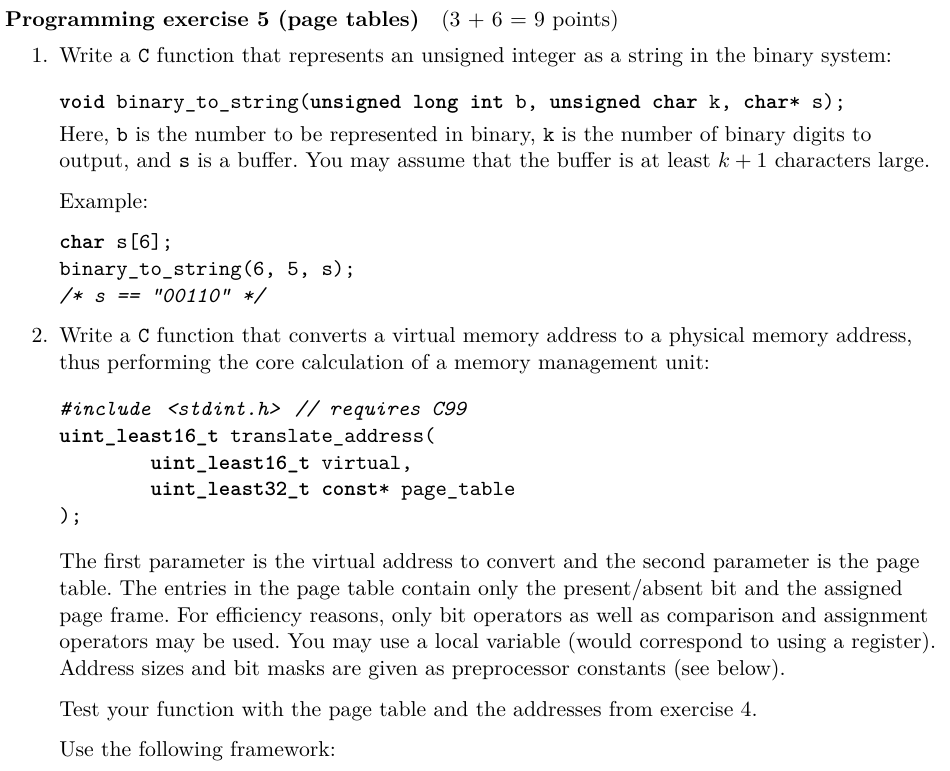
\includegraphics[keepaspectratio, width=\textwidth, height=\textheight-2\baselineskip]{img/104_ex5.png} \\
        \end{figure}
        \framebreak
        \begin{itemize}
         \item GLHF
         \item  \mintinline{c}{binary_to_string}
         \begin{itemize}
          \item iterate over the number of bits to represent
          \item What does this do? 
          \begin{minted}[autogobble]{c}
           ((b >> (k - 1 - i)) & 1);
          \end{minted}
        \end{itemize}
        \item \mintinline{c}{translate_address}
        \begin{itemize}
        \item you need to use bit shifts and binary ops
        \item Extract page table entry (using only the higher 16 - offset bits)
        \item If the 32nd bit in the entry is 0 it's a page fault
        \item else set the PA bit to 0 (e.g. by using \mintinline{c}{entry & ~PA_BIT}) and shift to the right place. 
        \item use virtual \& offset mask
        \item concat the two above 
        \end{itemize}
        \end{itemize}
\end{frame}

\section{References}
    \begin{frame}[allowframebreaks]
      \frametitle{References}
      \begin{tiny}
      \nocite{*}
      \printbibliography
      \end{tiny}
    \end{frame}


\end{document}
 
